
% This LaTeX was auto-generated from MATLAB code.
% To make changes, update the MATLAB code and republish this document.

\documentclass{article}
\usepackage{graphicx}
\usepackage{color}

\sloppy
\definecolor{lightgray}{gray}{0.5}
\setlength{\parindent}{0pt}

\begin{document}

    
    

\section*{6. Weierstrass Approximation Theorem}

\begin{verbatim}
ATAPformats
\end{verbatim}
\begin{par}

Every continuous function on a bounded interval can be approximated to
arbitrary accuracy by polynomials.  This is the famous Weierstrass
approximation theorem, proved by Karl Weierstrass when he was 70 years
old [Weierstrass 1885]. The theorem was independently discovered at about
the same time, in essence, by Carl Runge: as pointed out in 1886 by
Phragm\'en in remarks published as a footnote stretching over
four pages in a paper by Mittag-Leffler [1900], it can be derived as a
corollary of results Runge published in a pair of papers in 1885
[Runge 1885{\sc a} \& 1885{\sc b}].

\end{par} \vspace{1em}
\begin{par}
Here and throughout this book, unless indicated otherwise, $\|\cdot\|$ denotes the supremum norm on $[-1,1]$.
\end{par} \vspace{1em}
\begin{par}
\textbf{Theorem 6.1. Weierstrass approximation theorem.} \textit{Let $f$ be a continuous function on $[-1,1]$, and let $\varepsilon>0$ be arbitrary.  Then there exists a polynomial $p$ such that} $$ \| f-p \| < \varepsilon. $$ \textit{Outline of proof.}  We shall not spell out an argument in detail.  However, here is an outline of the beautiful proof from Weierstrass's original paper. First, extend $f(x)$ to a continuous function $\tilde f$ with compact support on the whole real line.  Now, take $\tilde f$ as initial data at $t=0$ for the diffusion equation $\partial u/\partial t = \partial^2u/\partial x^2$ on the real line.  It is known that by convolving $\tilde f$ with the Gaussian kernel $\phi(x) = e^{-x^2/4t}/\sqrt{4\pi t}$, we get a solution to this partial differential equation that converges uniformly to $f$ as $t\to 0$, and thus can be made arbitrarily close to $f$ on $[-1,1]$ by taking $t$ small enough. On the other hand, since $\tilde f$ has compact support, for each $t>0$ this solution is an integral over a bounded interval of entire functions and is thus itself an entire function, that is, analytic throughout the complex plane. Therefore it has a uniformly convergent Taylor series on $[-1,1]$, which can be truncated to give polynomial approximations of arbitrary accuracy. $~\hbox{\vrule width 2.5pt depth 2.5 pt height 3.5 pt}$
\end{par} \vspace{1em}
\begin{par}
For a fuller presentation of the argument just given as ``one of the most amusing applications of the Gaussian kernel,'' where the result is stated for the more general case of a function of several variables approximated by multivariate polynomials, see Chapter 4 of [Folland 1995].
\end{par} \vspace{1em}
\begin{par}

Many other proofs of the Weierstrass theorem
are also known, including these early ones:
\medskip
\hfill\break
\hbox{\kern .7cm}Runge (1885)
\hfill\break
\hbox{\kern .7cm}Picard (1891)
\hfill\break
\hbox{\kern .7cm}Lerch (1892 and 1903)
\hfill\break
\hbox{\kern .7cm}Volterra (1897)
\hfill\break
\hbox{\kern .7cm}Lebesgue (1898)
\hfill\break
\hbox{\kern .7cm}Mittag-Leffler (1900)
\hfill\break
\hbox{\kern .7cm}Fej\'er (1900 and 1916)
\hfill\break
\hbox{\kern .7cm}Landau (1908)
\hfill\break
\hbox{\kern .7cm}de la $\hbox{Vall\'ee}$ Poussin (1908)
\hfill\break
\hbox{\kern .7cm}Jackson (1911)
\hfill\break
\hbox{\kern .7cm}Sierpinski (1911)
\hfill\break
\hbox{\kern .7cm}Bernstein (1912)
\hfill\break
\hbox{\kern .7cm}Montel (1918)
\hfill\break
\vskip -5pt\par
For example, Bernstein's proof is a discrete analogue of
the argument just given: continuous diffusion is replaced by
a random walk made precise by the
notion of {\em Bernstein polynomials} (Exercise 6.4)
[Bernstein 1912{\sc D}].\ \ Lebesgue's proof, which appeared in his first paper published as
a student at age 23, is based on
reducing the approximation of general continuous functions to the
approximation of $|x|$ (Exercise 6.5) [Lebesgue 1898].  Fej\'er was an even younger
student, age 20, when he published his proof based on {\em Ces\`aro means}
(Exercise 6.6a) [Fej\'er 1900],
and he published a different proof years later based on {\em Hermite--Fej\'er
interpolation} (Exercise 6.6b) [Fej\'er 1916].
This long list gives an idea of
the great amount of mathematics stimulated by Weierstrass's theorem and
the significant role it played in the development of analysis in the
early 20th century.  For a fascinating presentation of this corner of
mathematical history, see [Pinkus 2000].

\end{par} \vspace{1em}
\begin{par}
Weierstrass's theorem establishes that even extremely non-smooth functions can be approximated by polynomials, functions like $x \sin(x^{-1})$ or even $\sin(x^{-1}) \sin(1/\sin(x^{-1}))$.  The latter function has an infinite number of points near which it oscillates infinitely often, as we begin to see from the plot below over the range $[0.07,0.4]$. In this calculation Chebfun is called with a user-prescribed number of interpolation points, 30,000, since the usual adaptive procedure has no chance of resolving the function to machine precision.
\end{par} \vspace{1em}
\begin{par}
 \vskip -2em 
\end{par} \vspace{1em}
\begin{verbatim}
f = chebfun(@(x) sin(1./x).*sin(1./sin(1./x)),[.07 .4],30000);
plot(f), xlim([.07 .4]), FS = 'fontsize';
title('A continuous function that is far from smooth',FS,9)
\end{verbatim}

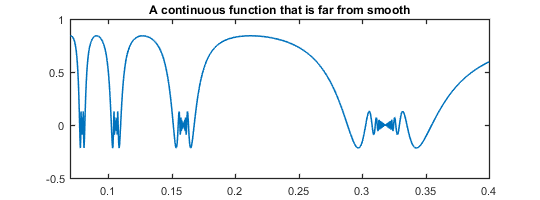
\includegraphics [width=4in]{chap6_01.png}
\begin{par}
 \vskip 1pt 
\end{par} \vspace{1em}
\begin{par}
We can illustrate the idea of Weierstrass's proof by showing the convolution of this complicated function with a Gaussian. First, here is the same function $f$ recomputed over a subinterval extending from one of its zeros to another:
\end{par} \vspace{1em}
\begin{par}
 \vskip -2em 
\end{par} \vspace{1em}
\begin{verbatim}
a = 0.2885554757; b = 0.3549060246;
f2 = chebfun(@(x) sin(1./x).*sin(1./sin(1./x)),[a,b],2000);
plot(f2), xlim([a b]), title('Close-up',FS,9)
\end{verbatim}

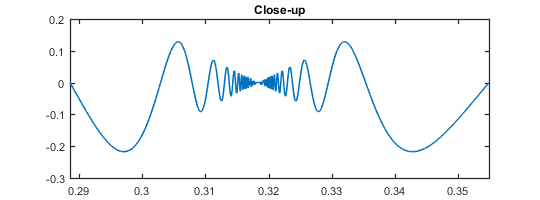
\includegraphics [width=4in]{chap6_02.png}
\begin{par}
 \vskip 1pt 
\end{par} \vspace{1em}
\begin{par}
Here is a narrow Gaussian with integral 1.
\end{par} \vspace{1em}
\begin{par}
 \vskip -2em 
\end{par} \vspace{1em}
\begin{verbatim}
t = 1e-7;
phi = chebfun(@(x) exp(-x.^2/(4*t))/sqrt(4*pi*t),.003*[-1 1]);
plot(phi), xlim(.035*[-1 1])
title('A narrow Gaussian kernel',FS,9)
\end{verbatim}

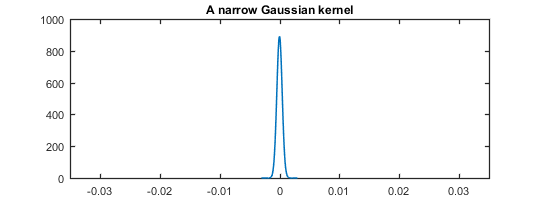
\includegraphics [width=4in]{chap6_03.png}
\begin{par}
 \vskip 1pt 
\end{par} \vspace{1em}
\begin{par}
Convolving the two gives a smoothed version of the close-up of $f$. Notice how the short wavelengths vanish while the long ones are nearly undisturbed.
\end{par} \vspace{1em}
\begin{par}
 \vskip -2em 
\end{par} \vspace{1em}
\begin{verbatim}
f3 = conv(f2,phi);
plot(f3), xlim([a-.003,b+.003])
title('Convolution of the two',FS,9)
\end{verbatim}

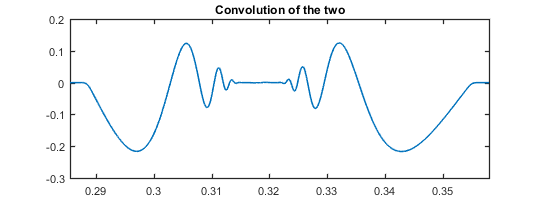
\includegraphics [width=4in]{chap6_04.png}
\begin{par}
 \vskip 1pt 
\end{par} \vspace{1em}
\begin{par}
This is an entire function, which means it can be approximated by polynomials by truncating the Taylor series.
\end{par} \vspace{1em}
\begin{par}

Weierstrass's theorem has
an important generalization to complex analytic functions.  Suppose
a function $f$ is defined on a compact set $K$ in the complex plane whose
complement is connected (so $K$ cannot have any holes).  {\em Mergelyan's
theorem} asserts that if $f$ is continuous on $K$ and analytic in the
interior, then $f$ can be approximated on $K$
by polynomials [Mergelyan 1951, Gaier 1987].
The earlier {\em Runge's theorem} is the weaker result in which $f$
is asumed to be analytic throughout $K$, not just in the
interior [Runge 1885{\sc a}].

\end{par} \vspace{1em}
\begin{par}
For all its beauty, power, and importance, the Weierstrass approximation theorem has in some respects served as an unfortunate distraction. Knowing that even troublesome functions can be approximated by polynomials, we naturally ask, how can we do it? A famous result of Faber and Bernstein asserts that there is no fixed array of grids of $1, 2, 3,\dots$ interpolation points, Chebyshev or otherwise, that achieves convergence as $n\to\infty$ for all continuous $f$ [Faber 1914, Bernstein 1919]. So it becomes tempting to look at approximation methods that go beyond interpolation, and to warn people that interpolation is dangerous, and to try to characterize exactly what minimal properties of $f$ suffice to ensure that interpolation will work after all. A great deal is known about these subjects. The trouble with this line of research is that for almost all the functions encountered in practice, Chebyshev interpolation works beautifully! Weierstrass's theorem has encouraged mathematicians over the years to give too much of their attention to pathological functions at the edge of discontinuity, leading to the bizarre and unfortunate situation where many books on numerical analysis caution their readers that interpolation may fail without mentioning that for functions with a little bit of smoothness, it succeeds outstandingly. For a discussion of the history of such misrepresentations and misconceptions, see Chapter 14 and also the appendix on ``Six myths of polynomial interpolation and quadrature.''
\end{par} \vspace{1em}
\begin{par}

\begin{displaymath}
\framebox[4.7in][c]{\parbox{4.5in}{\vspace{2pt}\sl
{\sc Summary of Chapter 6.}
A continuous function on a bounded interval can be approximated
arbitrarily closely by polynomials.\vspace{2pt}}}
\end{displaymath}

\end{par} \vspace{1em}
\begin{par}
 \smallskip\small\parskip=2pt
{\bf Exercise 6.1.  A pathological function of Weierstrass.} Weierstrass
was one of the first to give an example of a function continuous but
nowhere differentiable on $[-1,1]$, and it is one of the early examples
of a fractal [Weierstrass 1872]: $$ w(x) = \sum_{k=0}^\infty 2^{-k}
\cos(3^k x). $$ (a) Construct a chebfun {\tt w7} corresponding to this
series truncated at $k=7$.  Plot {\tt w7}, its derivative (use {\tt
diff}), and its indefinite integral ({\tt cumsum}).  What is the degree
of the polynomial defining this chebfun?  (b) Prove that $w$ is
continuous.  (You can use the Weierstrass M-test.)
\par
{\bf Exercise 6.2.  Taylor series of an entire function.} To illustrate
the proof of the Weierstrass approximation theorem, we plotted a Gaussian
kernel.  The key point of the proof is that this kernel is entire, so its
Taylor series converges for all $x$.  (a) For $x=1$ at the given time $t
= 10^{-7}$, how many terms of the Taylor series about $x=0$ would you
have to take before the terms fall below 1?\ \ Estimate the answer at least
to within a factor of 2.  You may find Stirling's formula helpful.  (b)
Also for $x=1$ and $t=10^{-7}$, approximately how big is the biggest term
in the Taylor series?
\par
{\bf Exercise 6.3.  Resolving a difficult function.} Although the
example function $f(x) = \sin(1/x)\sin(1/\sin(1/x))$ of this chapter
is not Lipschitz continuous, its Chebyshev interpolants do in fact converge.
Explore this phenomenon numerically by computing the degree $n$ Chebyshev interpolant
to $f$ over the interval $[0.07,0.4]$ for $n+1 = 4, 8, 16, \dots, 2^{14}$ and
measuring the error in each case over a Chebyshev grid of $2n$ points.
Plot the results on a loglog scale.  How do you think the error
depends on $n$ as $n\to\infty$?  Approximately how
large would $n$ have to be to get 16-digit accuracy
for this function over this interval?
\par
{\bf Exercise 6.4.  Bernstein's proof.}
For $f\in C([0,1])$, the associated degree $n$ {\em Bernstein polynomial}
is defined by
$$ B_n(x) = \sum_{k=0}^n f(k/n) {n\choose k} x^k (1-x)^{n-k}. \eqno (6.1) $$
Bernstein proved the Weierstrass approximation theorem by
showing that $B_n(x) \to f(x)$ uniformly as $n\to\infty$.
(a) Give an interpretation of $B_n(x)$ involving a random walk driven by a
coin which comes up heads with probability $x$ and tails with probability $1-x$.
(b) Show that $\max B_n(x) \le \max f(x)$ and $\min B_n(x) \ge \min f(x)$
for $x\in [0,1]$.
\par
{\bf Exercise 6.5.  Lebesgue's proof.}
(a) Show using uniform continuity that any $f\in C([-1,1])$
can be approximated uniformly by a polygonal curve, i.e., a function
$g(x)$ that is piecewise linear and continuous.
(b) Show that such a function can be written in the form
$ g(x) = A + Bx + \sum_{k=1}^m C_k |x-x_k|$.
(c) Show that $|x|$ can be uniformly approximated by polynomials on $[-1,1]$ by
truncating the binomial expansion
$$ [1-(1-x^2)]^{1/2} = \sum_{k=0}^\infty
{{1\over 2} \choose n} (x^2-1)^n . $$
You may use without proof the fact that these binomial coefficients
are of size $O(n^{-3/2})$ as $n\to\infty$.
(d) Explain how (a)--(c) combine to give a proof of the
Weierstrass approximation theorem.
\par
{\bf Exercise 6.6.  Fej\'er's proofs.}
(a) In 1900 Fej\'er proved the Weierstrass approximation theorem via
{\em Ces\`aro means}.  In the Chebyshev case, define $S_n$ to be the mean of
the partial sums of the Chebyshev series (3.11)--(3.12) of orders $0$ through
$n$.  Then $S_n\to f$ uniformly as $n\to\infty$ for any $f\in C([-1,1])$.
Explore such approximations for $f(x) = e^x$ with various degrees $n$.
For this very smooth function $f$, how does the accuracy compare
with that of ordinary Chebyshev interpolants?
(b) In 1916 Fej\'er proved the theorem again by considering
what are now known as {\em Hermite--Fej\'er interpolants}:
he showed that if $p_{2n}\in {\cal P}_{2n}$ is obtained by
interpolating $f\in C([-1,1])$ in the zeros of $T_n(x)$ and also setting
$p'(x)=0$ at these points, then $p_{2n}\to f$ uniformly as $n\to\infty$.
Explore such interpolants numerically for various $n$ by using \verb|interp1|
to construct polynomials $p_{2n}$ with
$p_{2n}(x_j) = p_{2n}(x_j+10^{-6}) = \exp(x_j)$.
Again how does the accuracy compare with that of ordinary Chebyshev
interpolants?
\par
{\bf Exercise 6.7.  Convergent series of polynomials.}
(a) Show that any $f\in C([-1,1])$ can be written as a uniformly
convergent series
$$ f(x) = \sum_{k=0}^\infty q_k(x), $$
where each $q_k$ is a polynomial of some degree.
(b) Show that a series of the same kind also exists for a function continuous on the
whole real line, with pointwise convergence for all $x$ and uniform
convergence on any bounded subset.
\par 
\end{par} \vspace{1em}



\end{document}
    
